%%%%%%%%%%%%%%%%%%%%%%%%%%%%%%%%%%%%%%%%%
% Short Sectioned Assignment LaTeX Template Version 1.0 (5/5/12)
% This template has been downloaded from: http://www.LaTeXTemplates.com
% Original author:  Frits Wenneker (http://www.howtotex.com)
% License: CC BY-NC-SA 3.0 (http://creativecommons.org/licenses/by-nc-sa/3.0/)
%%%%%%%%%%%%%%%%%%%%%%%%%%%%%%%%%%%%%%%%%

%----------------------------------------------------------------------------------------
%	PACKAGES AND OTHER DOCUMENT CONFIGURATIONS
%----------------------------------------------------------------------------------------

\documentclass[paper=a4, fontsize=10pt]{scrartcl} % A4 paper and 11pt font size

% ---- Entrada y salida de texto -----
\usepackage{ marvosym }

\usepackage[T1]{fontenc} % Use 8-bit encoding that has 256 glyphs
\usepackage[utf8]{inputenc}
%\usepackage{fourier} % Use the Adobe Utopia font for the document - comment this line to return to the LaTeX default

% ---- Idioma --------

\usepackage[spanish, es-tabla]{babel} % Selecciona el español para palabras introducidas automáticamente, p.ej. "septiembre" en la fecha y especifica que se use la palabra Tabla en vez de Cuadro

% ---- Otros paquetes ----

\usepackage{url} % ,href} %para incluir URLs e hipervínculos dentro del texto (aunque hay que instalar href)
\usepackage{amsmath,amsfonts,amsthm} % Math packages
%\usepackage{graphics,graphicx, floatrow} %para incluir imágenes y notas en las imágenes
\usepackage{graphics,graphicx, float} %para incluir imágenes y colocarlas

% Para hacer tablas comlejas
%\usepackage{multirow}
%\usepackage{threeparttable}

%\usepackage{sectsty} % Allows customizing section commands
%\allsectionsfont{\centering \normalfont\scshape} % Make all sections centered, the default font and small caps

\usepackage{fancyhdr} % Custom headers and footers
\pagestyle{fancyplain} % Makes all pages in the document conform to the custom headers and footers
\fancyhead{} % No page header - if you want one, create it in the same way as the footers below
\fancyfoot[L]{} % Empty left footer
\fancyfoot[C]{} % Empty center footer
\fancyfoot[R]{\thepage} % Page numbering for right footer
\renewcommand{\headrulewidth}{0pt} % Remove header underlines
\renewcommand{\footrulewidth}{0pt} % Remove footer underlines
\setlength{\headheight}{13.6pt} % Customize the height of the header

\numberwithin{equation}{section} % Number equations within sections (i.e. 1.1, 1.2, 2.1, 2.2 instead of 1, 2, 3, 4)
\numberwithin{figure}{section} % Number figures within sections (i.e. 1.1, 1.2, 2.1, 2.2 instead of 1, 2, 3, 4)
\numberwithin{table}{section} % Number tables within sections (i.e. 1.1, 1.2, 2.1, 2.2 instead of 1, 2, 3, 4)

\setlength\parindent{0pt} % Removes all indentation from paragraphs - comment this line for an assignment with lots of text

\newcommand{\horrule}[1]{\rule{\linewidth}{#1}} % Create horizontal rule command with 1 argument of height

% Añadidos por Rubén Morales Pérez
\usepackage[hidelinks]{hyperref} 
\usepackage[usenames]{color}
\usepackage{verbatim}
\usepackage{listings}
\usepackage{multicol}
\usepackage{caption}
\usepackage{subcaption}

\definecolor{Cyan}{RGB}{0,32,96}
\definecolor{codegreen}{rgb}{0,0.6,0}
\definecolor{codegray}{rgb}{0.5,0.5,0.5}
\definecolor{codepurple}{rgb}{0.58,0,0.82}
\definecolor{backcolour}{rgb}{0.95,0.95,0.92}

\lstdefinestyle{mystyle}{
	backgroundcolor=\color{backcolour},   
	commentstyle=\color{codegreen},
	keywordstyle=\color{magenta},
	numberstyle=\tiny\color{codegray},
	stringstyle=\color{codepurple},
	basicstyle=\footnotesize,
	breakatwhitespace=false,         
	breaklines=true,                 
	captionpos=b,                    
	keepspaces=true,                 
	numbers=left,                    
	numbersep=5pt,                  
	showspaces=false,                
	showstringspaces=false,
	showtabs=false,                  
	tabsize=2
}
\lstset{style=mystyle}



% Paquetes añadidos a la plantilla
\usepackage{anysize}
\marginsize{3cm}{3cm}{2.5cm}{2.5cm}
%\usepackage[scaled]{uarial}
% Para instalar la fuente seguir instrucciones de https://tex.stackexchange.com/questions/60644/latex-error-file-uarial-sty-not-found





%----------------------------------------------------------------------------------------
%	TÍTULO Y DATOS DEL ALUMNO
%----------------------------------------------------------------------------------------

\title{	
\normalfont \normalsize 
\textsc{\textbf{Ingeniería de Servidores (2016-2017)} \\ Grado en Ingeniería Informática \\ Universidad de Granada} \\ [25pt] % Your university, school and/or department name(s)
\horrule{0.5pt} \\[0.4cm] % Thin top horizontal rule
\huge IBM mainframes \\ Watson Machine Learning \\ % The assignment title
\horrule{2pt} \\[0.5cm] % Thick bottom horizontal rule
}

\author{Francisco Javier Morales Piquerasa
	\\ Rubén Morales Pérez} % Nombre y apellidos

\date{\normalsize\today} % Incluye la fecha actual

%----------------------------------------------------------------------------------------
% DOCUMENTO
%----------------------------------------------------------------------------------------

\begin{document}

\maketitle % Muestra el Título
\newpage %inserta un salto de página
\tableofcontents % para generar el índice de contenidos
\listoffigures
\listoftables

\newpage


\section{Resumen}
% Entre 5 y 15 líneas: 


\section{Memoria}
\subsection{Introducción}
Hay varios retos que tienen las compañías actualmente para poder mantenerse competitivas en un mundo cada vez más globalizado.
El mundo de las tecnologías de la información y la comunicación toma un papel fundamental, cada vez hay más corporaciones con página web, aplicaciones u ofreciendo información actualizada a través de redes sociales.

\

Una vez que tenemos una base tecnológica  y cierto volumen de negocio es recomendable pasar al siguiente nivel, tener datos suficientes y de calidad recopilados de forma que podamos obtener un beneficio competitivo extrayendo información.
Entonces entra en juego el análisis de datos y mantener esa información segura, por temas de protección de datos.
Aquí es donde interviene IBM mainframes \cite{ibm-m}, grandes ordenadores que nos ofrecen computación en la nube de forma que podremos almacenar los datos en dichos servidores con cierta garantía y a la vez dejar a estos ordenadores el procesamiento pesado.

\

El primer ordenador digital de propósito general de IBM fue ASCC (\href{https://www-03.ibm.com/ibm/history/exhibits/markI/markI_intro.html}{Automatic Sequence Controlled Calculator}), se desarrolló junto con la Universidad de Harvard. Entre los sistemas más modernos hablaremos de \href{https://www-03.ibm.com/systems/z/}{z Systems}.



\begin{figure}[H]
	\centering
	\begin{subfigure}{.5\textwidth}
		\centering
		\href{https://www-03.ibm.com/ibm/history/exhibits/markI/markI_intro.html}{		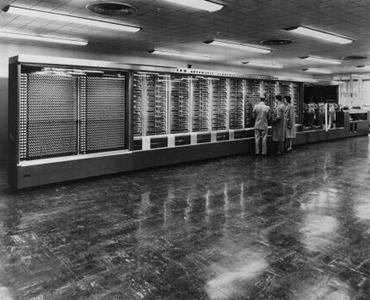
\includegraphics[width=.75\linewidth]{./Imagenes/ascc.jpg}}
		\caption{ASCC}
		\label{fig:ascc}
	\end{subfigure}%
	\begin{subfigure}{.5\textwidth}
		\centering
		\href{https://www-03.ibm.com/systems/z/hardware/z13.html}{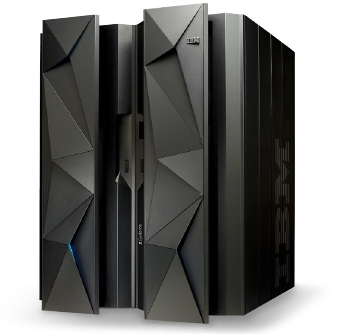
\includegraphics[width=.75\linewidth]{./Imagenes/z13.jpg}}
		\caption{Z13}
		\label{fig:z13}
	\end{subfigure}
\end{figure}



\subsection{IBM mainframes}
A día de hoy, los mainframes juegan un papel esencial en las operaciones diarias de las grandes compañías.
La era de la información reclama muchas innovaciones, y las grandes compañías son víctimas en la marcha implacable del progreso.
IBM desarrolla continuamente sus mainframes al mismo tiempo que mantiene la compatibilidad con aplicaciones existentes.

\

El término mainframe ha evolucionado gradualmente de una descripción física de las mayores computadoras de IBM hasta entenderse como un estilo de computación en sí mismo.
Un punto de inflexión en la historia de los mainframes fue el \textit{S/360}.
El desarrollo del mainframe empezó en una serie de generaciones en los años cincuenta.
En esa época eran las únicas computadoras y pocas empresas podían permitírselas, servían como repositorios de datos para las empresas.
En los años sesenta los fabricantes de mainframes comenzaron a estandarizar el hardware y el software que ofrecían a los clientes.

% The introduction of the IBM System/360™ (or S/360™) in 1964 signaled the start of the third generation: the first general purpose computers.
% En el otro enlace pone que el primero fue ASCC (?)


\subsubsection{Blockchain}
\subsection{Watson}
En 2007 \href{https://www.research.ibm.com/}{IBM Research} se propuso el reto de crear un sistema para competir con los grandes campeones en el juego \href{https://www.jeopardy.com/}{Jeopardy!}. 
Este sistema, en adelante Watson, entraría dentro de la categoría QA (Question answering), que requiere avances en varias áreas de la ciencia de la computación y la inteligencia artificial. 
Algunas de estas áreas serían búsqueda y recuperación de información (IR), procesamiento de lenguaje natural (NLP), representación del conocimiento y razonamiento o el machine learning.

\begin{figure}[H]
	\centering
	\label{j-watson}
	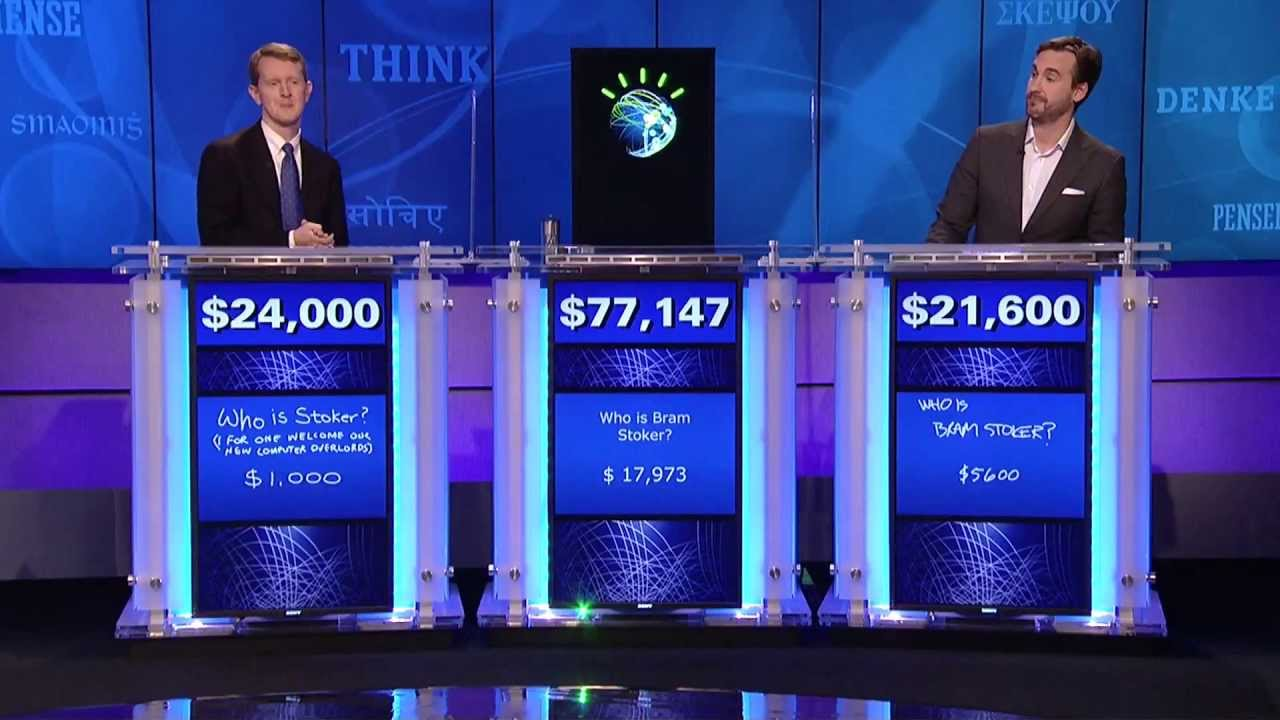
\includegraphics[width=0.8\textwidth]{./Imagenes/j-watson.jpg}
	\caption{Watson en Jeopardy!}
\end{figure}

\

La comunicación humana es imperfecta, está llena de ambigüedades, polisemia, ironías, la misma información puede darse de varias maneras y a veces la interpretación de una frase no solamente depende del contexto actual sino de conversaciones anteriores entre los interlocutores.
Además, dicha comunicación no está estructurada, como en un lenguaje de programación o una base de datos, donde los datos están bien definidos y la información es explícita.
A día de hoy la información no estructurada, como es el caso del lenguaje natural, crece más rápido que la estructurada, por ello es buena idea usar análisis profundos del lenguaje natural para hacer inferencia a partir de los datos de los que disponemos.
% this-is-watson: word-sense disambiguation [5, 6], latent semantic analysis [7], textual entailment [8], and coreference resolution [9]

\

Desde 2001 hasta 2006 se construyó la base para el reconocimiento de información no estructurada, UIMA (Unstructured
Information Management Architecture). % this-is-watson:[10]
UIMA proporciona una plataforma para integrar la información obtenida tras analizar textos, imágenes, etc.
Su objetivo es integrar varios programas llamados \textit{anotadores}, que asignan significado semántico a ciertas partes del texto o imagen.

% Watson was the system-level experiment that brought together hundreds of different cooperating algorithms, each of these algorithms alone performs relatively simple language processing tasks.
% In May 1997, IBM’s Deep Blue* computer beat Gary Kasparov (IBM Research beckoned for an encore)

Algunos desarrolladores habían participado anteriormente en Question answering dentro del proyecto PIQUANT \cite{piquant}. % this-is-watson [13, 14]
Este sistema tenía un conjunto estático de tipos de respuestas o clases de conceptos que se solicitaban en una pregunta.
El nuevo sistema no tendría conexión a Internet, y en unos tres segundos tendría que procesar la pregunta, buscar una respuesta y estimar la probabilidad de que sea correcta.
Tras analizar $2.000$ partidas de \textit{Jeopardy!} la media de los jugadores que ganaban era una precisión del $85-95\%$ de acierto sobre una media de $40-50\%$ de preguntas respondidas, o 
\textit{85\% Precision@40}


\subsubsection{Arquitectura}
En $2007$ se consiguió, usando PIQUANT, un rendimiento 16\% Precision@70 en las preguntas de \textit{Jeopardy!}.
Después se desarrollaron dos técnicas esenciales en el desarrollo de \textit{Watson}, DeepQA % this-is-watson: [4]
y AdaptWatson. % this-is-watson: [16,17]

\begin{figure}[H]
	\centering
	\label{tiw-deepqa}
	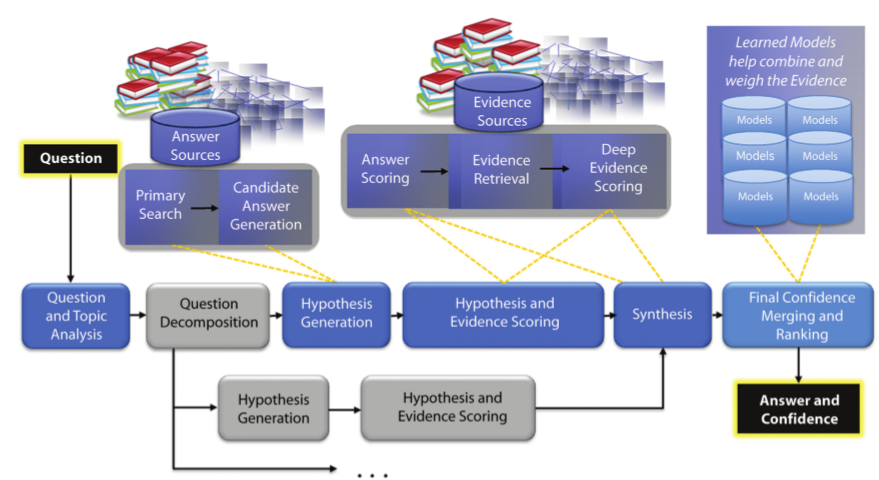
\includegraphics[width=0.8\textwidth]{./Imagenes/deepQA.png}
	\caption{Arquitectura DeepQA}
\end{figure}

\textbf{DeepQA} define varias etapas del análisis, cada una tiene diferentes implementaciones que se ejecutan en paralelo.  
Nunca se admite que se ha entendido perfectamente una pregunta, de forma que pueda verse directamente la respuesta en una base de datos.
Lo que se hace es buscar varias posibles preguntas candidatas, ponderar la probabilidad de que cada una sea la correcta, buscar varias posibles respuestas a cada pregunta y usar diferentes fuentes para ponderar la probabilidad de cada respuesta.
En dicho proceso se le da valor al hecho de que una respuesta concuerde con el tipo que se espera, por ejemplo un monumento histórico, una persona, etc.
También se tienen en cuenta fechas, geografía, la fiabilidad de las fuentes, etc.
Este análisis produce cientos de valores o características, cada uno indicando el grado de evidencia que se ha encontrado de cada tipo que refuerza una respuesta concreta.
Todas esas características deben ser combinados para obtener un único valor representando la probabilidad de que la respuesta sea correcta.
Para dar una ponderación a cada característica de DeepQA se entrenó con un modelo estadístico usando machine learning a partir de preguntas y respuestas.
% this-is-watson: [37]
El resultado final es una lista de respuestas candidatas, cada una con un valor que nos indica si es buena respuesta o no, en función de la evidencia.

\

El rendimiento del sistema no era demasiado alto, hasta que consiguieron integrar diferentes técnicas algorítmicas usando una metodología llamada \textbf{AdaptWatson}.
Estos componentes actúan sobre la arquitectura de DeepQA con el objetivo de entender las preguntas, buscar respuestas candidatas y ponderar la confianza en dichas respuestas.
El equipo documentó más de $8.000$ experimentos independientes en el ciclo de vida de Watson, cada uno con $10-20GB$ de datos.
A partir de estos datos se buscaban fallos y sus posibles causas.
De esta forma se mejoró hasta un 85\% Precision@70.

\subsubsection{Entendiendo las preguntas}
Una pregunta tiene un tipo de respuesta potencial que llamaremos LAT (lexical answer type), además cada pregunta en \textit{Jeopardy!} tiene una categoría que ayudará a identificar el tema sobre el que se pregunta. % this-is-watson: question analysis algorithms [18]
Para entender las preguntas formuladas se usa un parser ESG (English Slot Grammar) % this-is-watson: [19]
y un generador PAS (predicate-argument structure). 

\begin{itemize}
	\item ESG identifica partes de la frase y roles sintácticos como el sujeto y relaciones entre las diferentes partes de la frase.
	\item El generador PAS es usado para producir una representación abstracta, que representa la interfaz con la parte analítica (otra capa de DeepQA de la resolución del problema.
\end{itemize}

En cuanto a las \textbf{respuestas y fuentes de evidencia} al principio se usaba añadieron enciclopedias y libros de referencia. Después se desarrolló un proceso semiautomático para hacer crecer el conocimiento de Watson, no se puede añadir contenido sin parar ya que afecta al rendimiento del sistema.
% this-is-watson: proceso para añadir conocimiento [20, 21]
Tras analizar el contenido que se añade se crea PRISMATIC, que extrae información y usa la estadística para deducir lo que es conocimiento base, esto ayudará en la parte de generación de respuestas candidatas y calcular sus probabilidades.
% this-is-watson: descubrir respuestas candidatas [22]

\

Cada una de las consultas usan información estructurada y no estructurada usando varios mecanismos de búsqueda complementarios.
Una pareja de consulta y respuesta representan una hipótesis.
% this-is-watson: generación de hipótesis [23]
Una métrica %(candidate binary recall)
que se usa para medir la bondad de una respuesta es el porcentaje de preguntas en las que dicha respuesta es generada como candidata. 
Esta medida ayuda a combinar los resultados, sobre todo cuando tenemos varias interpretaciones diferentes de lo que se está preguntando.
De esta forma se determina la probabilidad final de que una respuesta sea correcta para la pregunta inicial.
De las experiencias de los desarrolladores con el sistema PIQUANT sabían que no era una estrategia adecuada intentar anticipar todos los tipos de respuesta y crear algoritmos que busquen solamente instancias de dichas clases.
Esto es debido en parte a la complejidad de algunas preguntas, ya que todo el sistema se apoya en haber reconocido correctamente el tipo de respuesta necesaria, y que en el conocimiento del sistema dicha respuesta esté bien clasificada.
En la siguiente pregunta de la categoría \textit{decoración} el tipo de respuesta buscada es una \textit{dirección}:

\begin{center}
Si usted está de pie, es la dirección que debe buscar para ver el revestimiento.

\textbf{Respuesta}: Abajo
\end{center}

\

Para clasificar las respuestas se usó un sistema dinámico que tenía en cuenta el contexto de la pregunta, su nombre es \textit{coacción de tipo}. % this-is-watson: [24, 27]
Otras técnicas técnicas usadas por Watson eran PRISMATIC, YAGO y WordNet. % this-is-watson [21, 25, 26]
Otra fase del proceso es \textbf{recolectar y evaluar la evidencia} (o refutación) acerca de las respuestas. 
Cada una de las búsquedas de evidencia se puede procesar paralelamente.
% this-is-watson: extracción dinámica de tipos [29]
En la búsqueda de tipos se utiliza la deducción de relaciones a partir de datos de entrenamiento de los que se extraen relaciones semánticas. Por ejemplo, esta pregunta de la categoría \textit{Madres e hijos}:

\begin{center}
Aunque solo les separa un año de vida, ella interpretó a la madre de Colin Farrell en Alexander

\textbf{Respuesta}: Angelina Jolie

\textbf{Relación}: protagoniza(ella, Alexander)
\end{center}

\

En Jeopardy! hay preguntas que tienen referencias implícitas en la frase, y unas partes del enunciado pueden depender de otras, como en el siguiente ejemplo de la categoría \textit{Antes y después}:

\begin{center}
La estrella de Jerry Maguire que mantiene automáticamente la velocidad de tu vehículo

\textbf{Respuesta}: Control Tom Cruise
\end{center} 

Hay una serie de algoritmos que primero detectan este tipo de preguntas y las referencias enlazadas en las frases.
Hay veces que interesa conocer la relación entre varias entidades, o aquello que tienen en común.
Para interpretar las preguntas se dividen en distintas partes lógicas que puedan ser exploradas independientemente y combinar los resultados. % this-is-watson: [36]
Por ejemplo, en esta pregunta con categoría \textit{Animales ficticios}, el sistema puede buscar por un lado personajes introducidos en $1894$ y por otro 

\begin{center}
El nombre de este personaje, introducido en $1894$, proviene de $"$Hindi for bear$"$

\textbf{Respuesta}: Baloo
\end{center}

\

Para poder ser operativo en un juego, el sistema debe mejorar las $2$ horas de procesamiento que necesita para responder una pregunta (en $2008$).
El $UIMA-AS$ permite a cualquier aplicación $UIMA$ ser desplegada en una colección de procesos asíncronos que usan paso de mensajes para comunicarse.
Cada pregunta se interpreta en un determinado número de preguntas candidatas, cada una se ejecuta independientemente, cada respuesta potencial de una pregunta candidata se ejecuta independientemente, y cada parte de evidencia también.
Tras usar $2880$ procesadores la latencia de respuesta bajó de dos horas a tres segundos. % this-is-watson [39]

\

Este sistema de pregunta-respuesta es estático y no aprovecha todo el potencial de la arquitectura DeepQA.
Watson puede aplicarse a la salud modificando su base de conocimiento y enseñándole a hacer las preguntas adecuadas a los pacientes para obtener información sobre ellos e inferir una solución a partir de su historial médico.




\section{Conclusiones}




%------------------------------------------------
\newpage
\bibliography{citas} %archivo citas.bib que contiene las entradas 
\bibliographystyle{plain} % hay varias formas de citar

\end{document}
